	\setlength{\abovedisplayskip}{0em}
	\setlength{\belowdisplayskip}{0em}
	
	\section*{一、问题求解}
	
	\textbf{问题求解}:通过一序列行动来达到目标
	
	\textbf{搜索}:寻找行动序列的过程
	
	\textbf{无/有信息搜索}:是否使用状态空间外的信息
	
	\textbf{约束满足}:
	
	\textbf{对抗搜索}:
	
	\subsection*{状态空间(状态集,行动集,代价函数)}
	
	\textbf{状态}:问题的某种情况(初始、目标、中间),表达方式多样
	
	\textbf{行动}:状态转换($S_i \rightarrow S_j, OP(\text{操作对象,初值,终值})$)
	
	\textbf{代价}:行动的开销($COST(O, S_i, S_j)$)
	
	例食人生番:动作op(b1,b2,b3)(人数,野人数,哪岸到哪岸)
	状态(a1,a2,a3)(左岸人num,左岸野人num,船在左or右)
	
	\subsection*{状态空间的数据结构}
	
	\textbf{深度}:节点到树根的路径长度
	
	\textbf{祖先/子孙}:包含自己,"真"才去掉
	
	\textbf{状态空间图}:状态-节点,动作-边,代价-权重
	
	\subsection*{无信息搜索}
	
	\textbf{宽搜}:经典图搜索;开节点表(检测到还没去进一步搜的点)用queue,闭节点表(搜过的点)用set;流程:开表取出点进一步搜,该点入闭表,新检测到的点入开表;完备性、最优性、时空均指数复杂度
	
	\textbf{一致代价搜索}:考虑路径代价的图搜索;每次扩展路径代价最小的子节点;开节点表用优先队列;额外操作:如果扩展使开节点表中节点代价变小,则应更新其代价;要求:单步代价非负,不存在代价0的环路;完备、最优时空均指数复杂度
	
	\textbf{深搜}:经典树搜索;开节点表用stack,闭节点表不需要;仅在树上有完备性,无最优性,时间指数复杂度,空间线性复杂度
	
	\textbf{深度受限搜索}:
	
	\textbf{迭代加深搜索}:不断增加深度限制;完备性、最优性、时间指数复杂度、空间线性复杂度
	
	\subsection*{有信息搜索}
	
	\textbf{启发函数}:当前状态与目标状态距离的函数$h(n)$(不可为负)
	
	\textbf{贪婪最佳优先搜索}:把一致代价搜索的代价函数换为$h(n)$;完备性、无最优性、时空均指数复杂度(实际较低,有效分支因子通常较小)
	
	\textbf{A*算法}:$f(n)=g(n)+h(n)$,均非负;有完备性,最优性见下,时空均指数复杂度,仅进行了剪枝
	
	\textbf{可采纳性}:$h(n)<$真实代价$\rightarrow$树搜索最优性
	
	\textbf{一致性}:$h(n)$满足三角不等式$\rightarrow$图搜索最优性(沿任何路径的f(n)值非递减)
	
	\textbf{占优}:称$h_2$比$h_1$占优,若$\forall n~h_1(n) \le h_2(n)$ $\rightarrow$ 计算量允许时,用更大的启发函数
	
	\textbf{设计启发函数}:1. 松弛问题(放宽条件),保证可采纳性和一致性;2.启发函数合成:$h(n)=max\{h_1(n), h_2(n), ... h_k(n)\}$;3.求解子问题:屏蔽掉状态中的一些变量,以简单的子问题的解作为启发函数;4.模式数据库:预先算好一些特定情况的解,以此推断启发函数;5.从经验学习:通过已经求结果的问题推断问题可能的解
	
	\subsection*{约束满足问题}
	
	\textbf{问题的原子表示}:把状态当黑盒,不引入内部信息
	
	\textbf{要素化表示}:利用状态内元素的依赖/制约关系(例八皇后)$\downarrow$
	
	\textbf{用一组变量描述状态}:$\mathbf{X}=\{X_1,...,X_n\}$,并写出$X_i$的含义
	
	\textbf{值域}:$\mathbf{D}=\{D_1,...,D_n\}, X_i \in D_i$
	
	\textbf{约束}:$\mathbf{C}=\{\text{约束变量}, \text{满足条件}\}$
	
	\textbf{离散型/连续型}:按值域特征分类
	
	\textbf{一元/二元/全局约束}:每组约束变量个数
	
	\textbf{求解过程}:搜索+推理交替$\downarrow$
	
	\textbf{节点相容}:称$X_i$节点相容,若$\forall x_i \in D_i$,$X_i=x_i$满足$X_i$的一元约束;若$\forall X_i$节点相容,则称该约束网络节点相容
	
	\textbf{边相容}:称$X_i$边相容,若$\forall x_i \in D_i$可以满足与$X_i$的所有二元约束($X_j$只需存在);若$\forall X_i$边相容,则称该约束网络$\sim$【检测算法AC-3:不断删除值域中不满足边相容的值,如果一个变量的值域在检测过程中发生了变化,则应重新检测与之相关的所有边,若有变量值域为空,则待求解问题无解】
	
	\textbf{路径相容}3-相容:对$X_3$能够找到一个与$X_1$和$X_2$相容的值
	
	\textbf{全局约束}:例Alldiff约束,可化简至无单值变量
	
	\textbf{约束问题中的搜索}:理解为尝试的过程,尝试有策略$\downarrow$
	
	\textbf{变量选择的顺序}:静态选择、最少剩余值、最多约束项
	
	\textbf{取值选择的顺序}:最少约束值(让邻居能选的值更多;找所有解或问题无解时无所谓)
	
	\textbf{搜索中的推理}:变量赋值后进行边相容检查
	
	\textbf{智能回溯}:需要回溯时,退回到产生冲突的变量,而非上一个变量
	
	\textbf{局部搜索}:从随机初始状态逐步改进直到发现解(可能卡住);优势:时空效率高,能用于大规模、无限/连续状态空间求解
	
	\textbf{最小冲突数法}:随机选一个有冲突的变量改,使冲突数最少
	
	\textbf{爬山法}:贪婪局部搜索,不断转移到邻近的更好状态,可获最优解/陷入局部最优
	
	\textbf{爬山法改进策略}:随机移动、随机重启、模拟退火(以一定概率允许下山)、局部束搜索(多个状态同步进行)
	
	\subsection*{对抗搜索-博弈}
	
	\textbf{博弈树}:与或树(赢1输0,我方或max,对方与min)
	
	\textbf{极大极小搜索}:我方取后继的max,对方取后继的min;时空复杂度同深搜
	
	\textbf{$\alpha-\beta$剪枝}:深搜;$\alpha$是max的下界,$\beta$是min的上界
	
	·$\alpha : \beta \text{(后继层)} \leq \alpha \text{(先辈层),}\text{终止该} \mathrm{MIN} \text{层后续搜索}$
	
	·$\beta : \alpha \text{(后继层)} \geq \beta \text{(先辈层),}\text{终止该} \mathrm{MAX} \text{层后续搜索}$
	
	类比:犯罪团伙-犯罪嫌疑人-受害者,max-min-max,施害过程是$\alpha$剪枝,因为min只能变小了,不比幕后者当前$\alpha$优
	
	优化效果:分支因子从b变为$b^{1/2}$,相同时间搜2倍步数
	
	\section*{二、逻辑推理}
	
	\subsection*{命题逻辑}
	·逻辑联结词:$ \wedge $(合取), $ \vee $(析取), $ \rightarrow $(蕴含), $ \leftrightarrow $(等价)
	
	·蕴含规则:$ p\rightarrow q $为假当且仅当$ p=T,q=F $
	
	·公式分类:永真式(重言式)、永假式(矛盾式)、可满足式(至少一个成真赋值)
	
	·吸收律:
	$ A\vee(A\wedge B)\Leftrightarrow A $
	$ A\wedge(A\vee B)\Leftrightarrow A $
	$ A\vee(B\wedge C)\Leftrightarrow(A\vee B)\wedge(A\vee C) $
	
	·德摩根律:$\sim(A\vee B)=\sim B\wedge\sim A$, $\sim(A\wedge B)=\sim B\vee\sim A$
	
	·重要等价式:
	$ A\rightarrow B\Leftrightarrow\sim A\vee B $
	$ (A\rightarrow B)\wedge(A\rightarrow\sim B)\Leftrightarrow\sim A $
	$ A\leftrightarrow B\Leftrightarrow(A\rightarrow B)\wedge(B\rightarrow A) $
	
	\subsection*{谓词逻辑}
	·量词转换:
	
	$\sim(\forall x)P(x)\Leftrightarrow(\exists y)\sim P(y)$
	
	$\sim(\exists x)P(x)\Leftrightarrow(\forall y)\sim P(y)$
	
	·分配律:
	
	$ (\forall x)(P(x)\wedge Q(x))\Leftrightarrow(\forall x)P(x)\wedge(\forall x)Q(x) $
	
	$ (\exists x)(P(x)\vee Q(x))\Leftrightarrow(\exists x)P(x)\vee(\exists x)Q(x) $
	
	·前束范式:将量词提到公式最左边
	
	·Skolem标准型:$\forall x\exists yP(x,y)\to\forall xP(x,f(x))$
	
	\subsection*{基于规则的推理}
	·逆向演绎系统:
	
	规则转换:$W\rightarrow L$(结论推条件)
	
	示例:目标$CAT(x)\wedge DOG(y)\wedge \text{AFRAID}(x,y)$,通过$\{x5/x\}$等置换推导
	
	·产生式系统:
	
	三要素:控制策略、产生式规则、总数据库
	
	规则库要求:完整性、一致性、准确性
	
	\section*{三、监督学习}
	
	\subsection*{线性回归+最小二乘法}
	
	\textbf{流程}:找线性函数族$y=wx+b~\rightarrow$确定优化目标:最小化平方损失$L(w,b)=\sum_{i=1}^{n}\left(y_{i}-\left(wx_{i}+b\right)\right)^{2}~\rightarrow$最优函数
	
	$\textstyle S_{xx} = \sum\left(x_{i} - \bar{x}\right)^{2}, 
	S_{xy} = \sum\left(x_{i} - \bar{x}\right)\left(y_{i} - \bar{y}\right), 
	S_{yy} = \sum\left(y_{i} - \bar{y}\right)^{2}$
	
	$\hat{\omega} = \frac{S_{xy}}{S_{xx}} 
	= \frac{\sum x_{i}y_{i} - n\bar{x}\bar{y}}{\sum x_{i}^{2} - n\bar{x}^{2}} 
	= \frac{S_{xy}}{S_{xx}}, \hat{b} = \bar{y} - \hat{\omega}\bar{x}$
	
	\textbf{平方和分解性质}$\sum (y_i - \bar{y})^2 = \sum (\hat{y}_i - \bar{y})^2 + \sum (y_i - \hat{y}_i)^2, SST=SSR+SSE$
	
	\textbf{确定系数} $R^2 = \frac{\sum (\hat{y}_i - \bar{y})^2}{\sum (y_i - \bar{y})^2} = \frac{SSR}{SST}$
	
	\textbf{测试方法}:独立测试集;随机抽样;交叉验证
	
	\textbf{评价指标}:$\text{平均绝对误差MAE} = \frac{1}{n} \sum_{i=1}^{n} |y_i - \hat{y}_i|, \text{MSE} = \frac{1}{n} \sum_{i=1}^{n} (y_i - \hat{y}_i)^2$, $\text{RMSE} = \sqrt{\frac{1}{n} \sum_{i=1}^{n} (y_i - \hat{y}_i)^2}$
	
	\textbf{多项式回归}:$y = w_0 + w_1 x + w_2 x^2 + \cdots + w_d x^d$
	
	$$
	\mathbf{y} = X\mathbf{w}, \quad
	X = \begin{bmatrix}
		1 & x_1 & x_1^2 & \cdots & x_1^d \\
		1 & x_2 & x_2^2 & \cdots & x_2^d \\
		\vdots & \vdots & \vdots & \ddots & \vdots \\
		1 & x_n & x_n^2 & \cdots & x_n^d
	\end{bmatrix}, \quad
	\mathbf{w} = \begin{bmatrix}
		w_0 \\ w_1 \\ \vdots \\ w_d
	\end{bmatrix}
	$$
	
	最小二乘解:$\mathbf{w}^* = \arg\min_{\mathbf{w}} \lVert \mathbf{y} - X\mathbf{w} \rVert^2 = (X^\top X)^{-1} X^\top \mathbf{y}$
	
	\textbf{多元线性回归}:形式几乎一致
	
	\textbf{容量}:模型拟合函数的能力
	
	\textbf{简单模型}:偏差大、方差小,容易欠拟合
	
	\textbf{复杂模型}:偏差小、方差大,容易过拟合
	
	\textbf{欠拟合}:用更复杂的模型
	
	\textbf{过拟合}:增加训练数据量;用更简单的模型
	
	\subsection*{Logistic回归}
	
	\textbf{二分类问题}:$\{\mathbf{x}_i, y_i\}, y_i \in \{0, 1\}$
	
	\textbf{Logistic函数(Sigmoid函数)}:$\sigma(x) = \frac{1}{e^{-x}}$
	
	$P(Y=1 \mid x) = \pi(x) = \frac{1}{1 + e^{-(w^T x + b)}} = \sigma(w^T x + b)$
	
	$P(Y=0 \mid x) = 1 - P(Y=1 \mid x) = \frac{e^{-(w^T x + b)}}{1 + e^{-(w^T x + b)}}$
	
	\textbf{几率比}:$\frac{P(Y=1 \mid x)}{P(Y=0 \mid x)} = e^{w^T x + b}$
	
	\textbf{对数几率}:$\log \frac{P(Y=1 \mid x)}{P(Y=0 \mid x)} = w^T x + b$,线性,可解释性强:$w$是$x$增加一个单位时对数几率的变化量;$exp(w)$表示x+1与x处的几率比为常数
	
	\textbf{优化目标}:似然函数$	L(w, b) = \prod_{i=1}^n P(Y=y_i) = (\pi(x_i))^{y_i}(1-\pi(x_i))^{1-y_i}$,对数似然$l(w,b)=\sum_{i=1}^{n}(y_i log \pi(x_i)+(1-y_i)log(1-\pi(x_i))$,交叉熵损失多一个-(1/n),本质一样
	
	数学表达$\min - \mathbb{E}_{(X,Y) \in \mathcal{D}} \left[ Y \log \pi(X) + (1 - Y) \log(1 - \pi(X)) \right]$
	
	\textbf{求解方法}:随机梯度下降(SGD),每次只需算一个样例
	
	\textbf{前向传播}:$z = w x + b,~\pi = h(z) = \frac{e^{z}}{1 + e^{z}} = \frac{1}{1 + e^{-z}}, ~e = J(\pi) = -y \log \pi - (1 - y) \log(1 - \pi)$
	
	\textbf{梯度计算}:$\frac{\partial e}{\partial b} = \frac{de}{d\pi} \frac{d\pi}{dz} \frac{\partial z}{\partial b} = \frac{\pi - y}{\pi(1 - \pi)} \cdot \pi(1 - \pi) = \pi - y$
	
	$\frac{\partial e}{\partial w} = \frac{de}{d\pi} \frac{d\pi}{dz} \frac{\partial z}{\partial w} = \frac{\pi - y}{\pi(1 - \pi)} \cdot \pi(1 - \pi) \cdot x = (\pi - y)x$
	
	\textbf{更新}:$x^{(new)} \leftarrow x-\alpha f'(x)$
	
	\textbf{二分类评价指标}:
	
	\begin{figurehere}
		\centering
		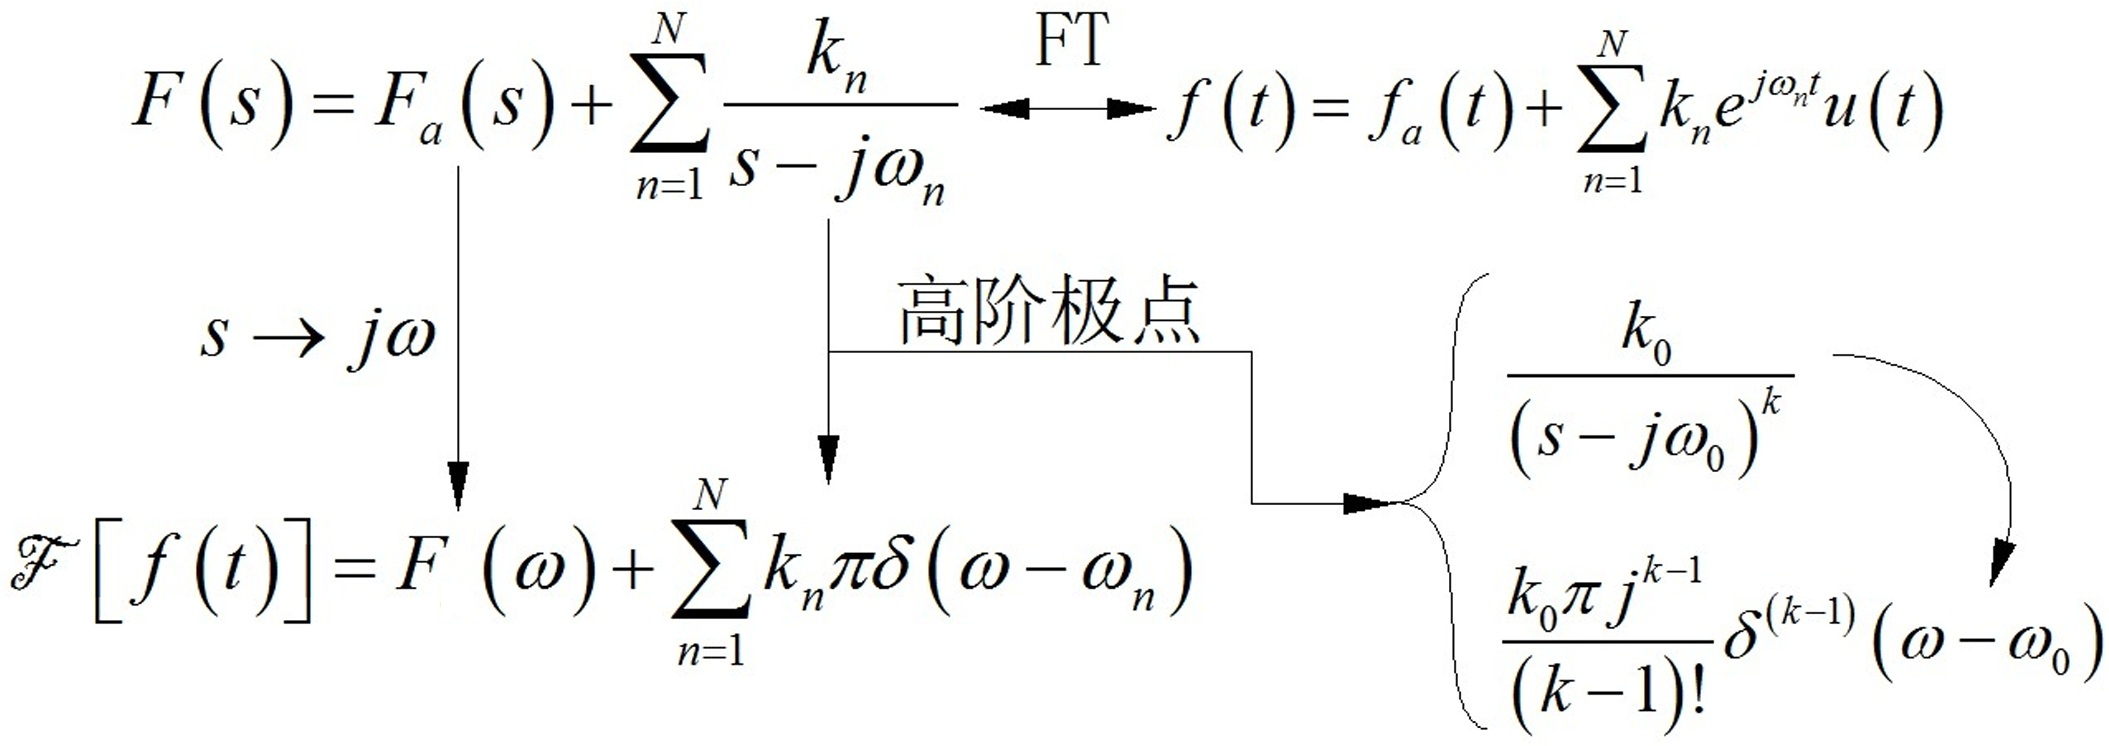
\includegraphics[width=0.6\linewidth]{image01}
		\label{fig:image01}
	\end{figurehere}
	
	\begin{figurehere}
		\centering
		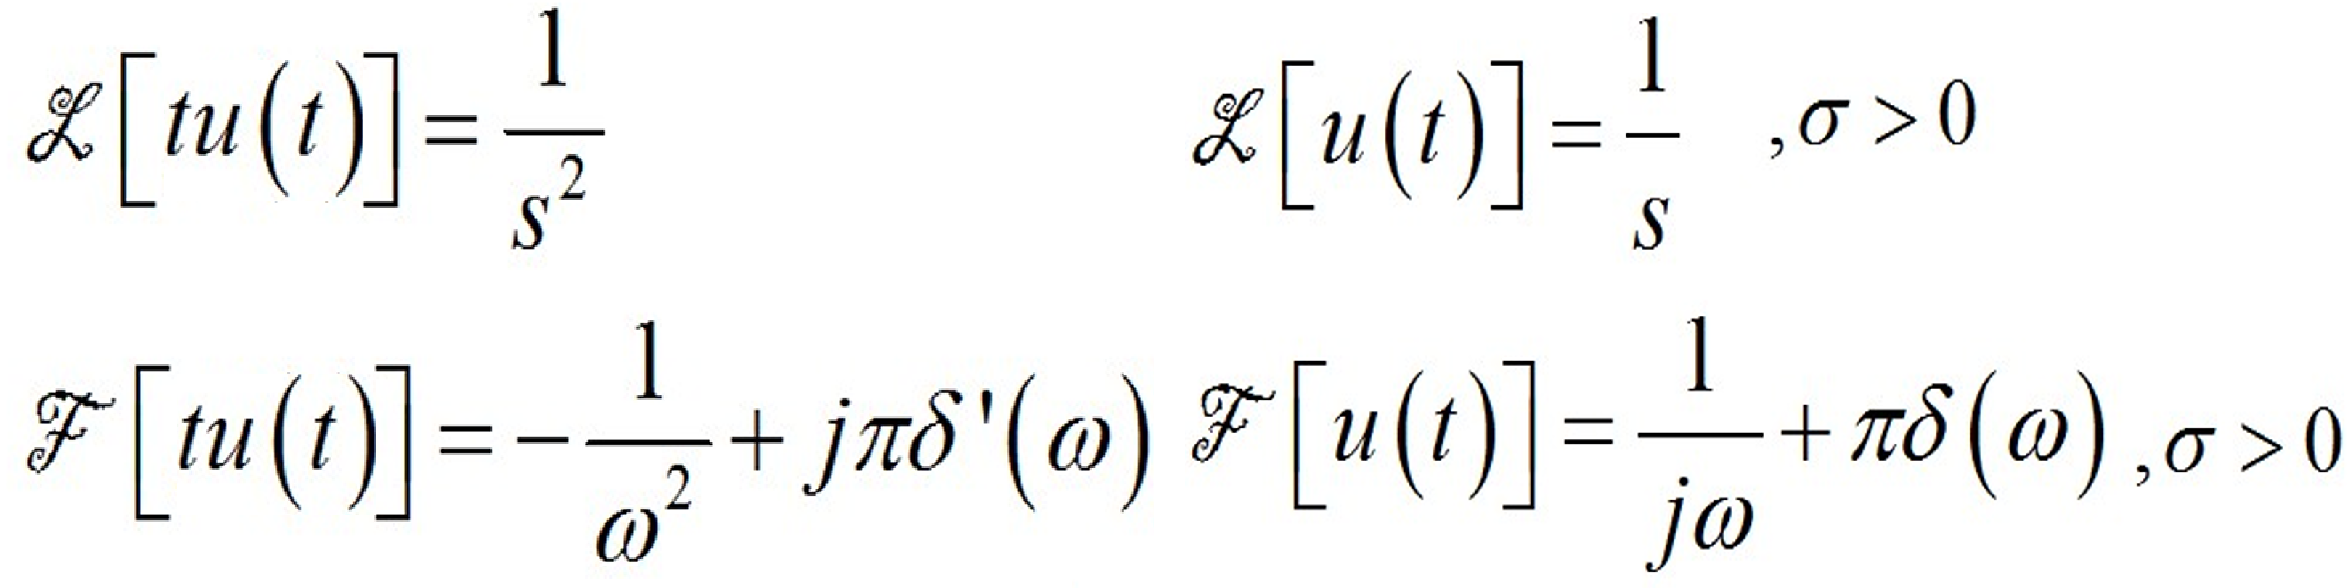
\includegraphics[width=1\linewidth]{image02}
		\label{fig:image02}
	\end{figurehere}
	\textbf{ROC曲线}:假阳性-真阳性,从0开始曲线爬升得越快,说明模型得性能越好,AUC越大模型性能越好
	
	\textbf{PRC曲线}:召回率-精确率,靠上性能好,auPRC越大越好
	
	\subsection*{Softmax回归}
	
	\begin{figurehere}
		\centering
		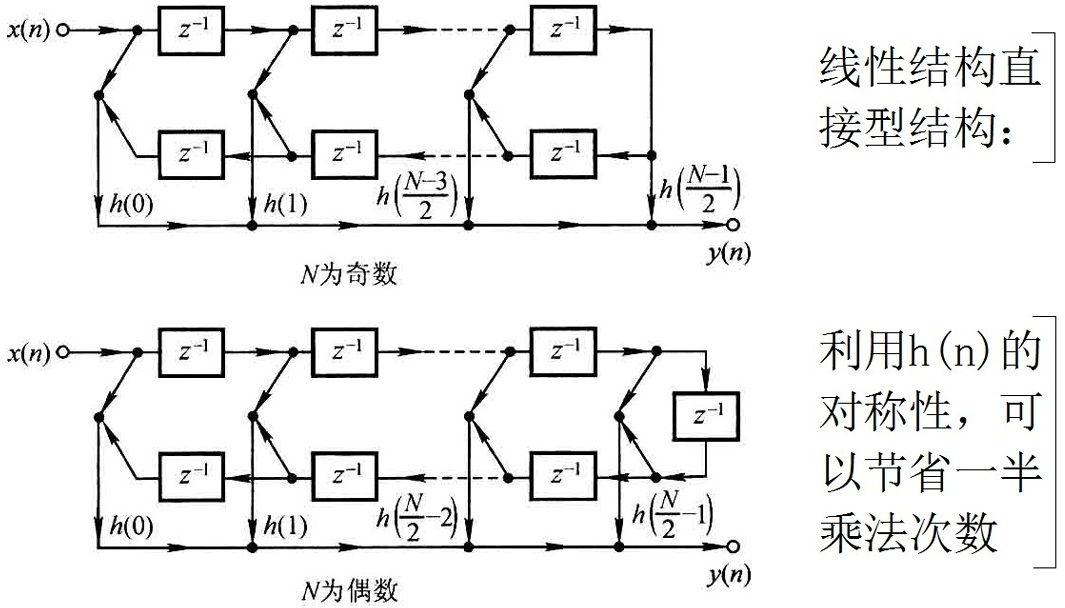
\includegraphics[width=1\linewidth]{image03}
		\label{fig:image03}
	\end{figurehere}
	\textbf{多分类评价指标}:微观指标(先整合类别再计算指标)、宏观指标(先计算指标再整合类别)
	
	\subsection*{前馈神经网络}
	
	\textbf{神经元}:输入向量$\mathbf{x}=(x_i)_{m\times1}$,输出标量$a$,线性整合$z=\mathbf{w}^T\mathbf{x}+b$(权重、偏执),激活$a=h(z)$,神经元的差异主要由激活函数决定
	
	\textbf{前馈神经网络}:分层图,n层神经网络第0层是输入层,1$\sim$-1层是隐含层,第n层是输出层,上标$^[k]$表示
	
	\textbf{输出层}:回归-线性单元,二分类-Logistic,多分类-Softmax
	
	\begin{figurehere}
		\centering
		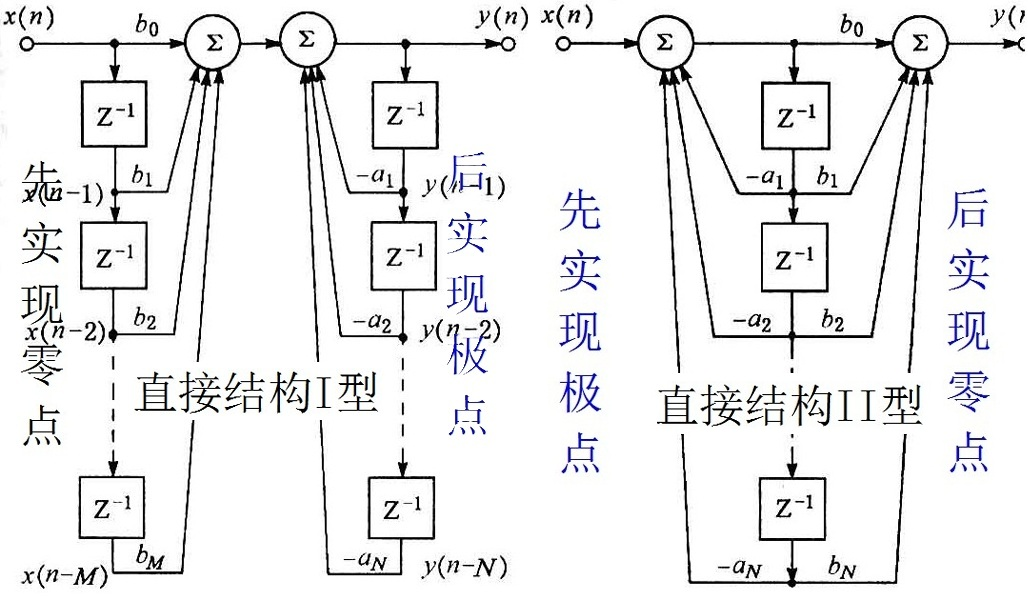
\includegraphics[width=1\linewidth]{image04}
		\label{fig:image04}
	\end{figurehere}
	\textbf{隐层}:线性单元、Logistic单元、$\downarrow$
	
	\begin{figurehere}
		\centering
		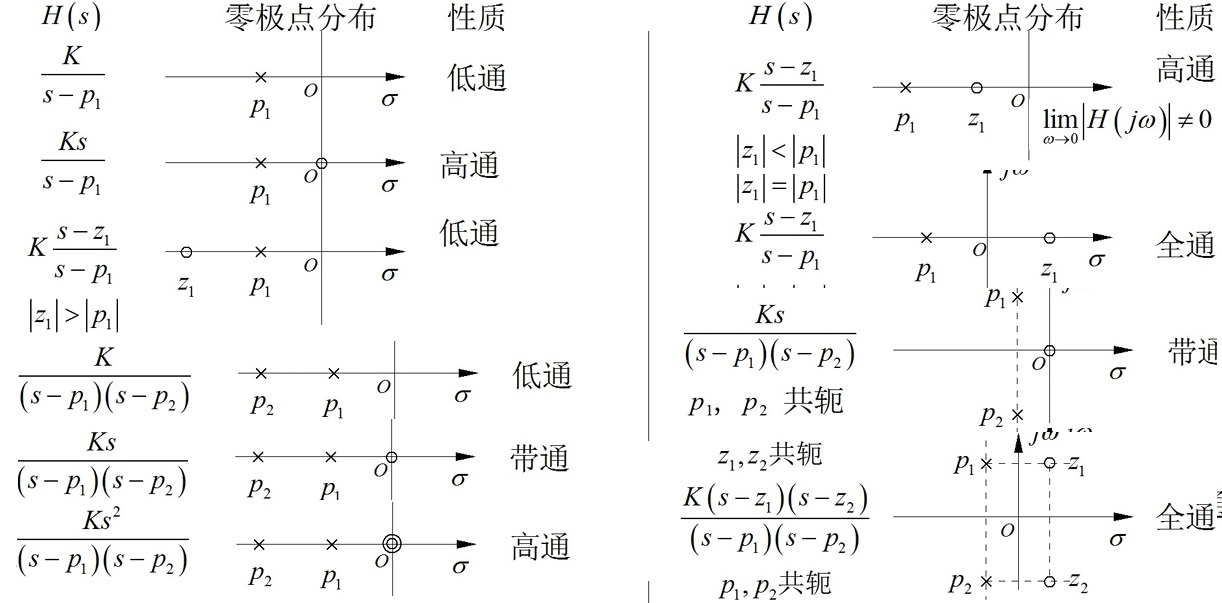
\includegraphics[width=1\linewidth]{image05}
		\label{fig:image05}
	\end{figurehere}
	\textbf{网络结构设计}:可表示区域的数量$O(k^m*C\{k\}\{m\}^{m(d-1)})$,深的网络性能好
	
	\subsection*{卷积神经网络}
	
	\textbf{填充}:same padding周边填0;valid padding不允许超出边界
	
	\textbf{步长}:步长>1时,卷积后矩阵显著变小
	
	特征:\textbf{稀疏连接、参数共享、等变表示}:全连接参数量$O(N^2)$vs卷积核参数量$O(m^2)$连接数$O(Nm^2)$,卷积核尺寸$m\ll N$
	
	\textbf{池化}:用某一位置相邻输出的统计特征作为该位置的输出
	
	\textbf{池化函数}:最大池化/平均池化/随机池化
	
	·步长大于1的池化能够降低输入规模
	
	\subsection*{循环神经网络}
	
	\textbf{序列输入}:长度不固定,上下文相关
	
	\textbf{困难}:梯度消失、长期依赖消失
	
	\begin{figurehere}
		\centering
		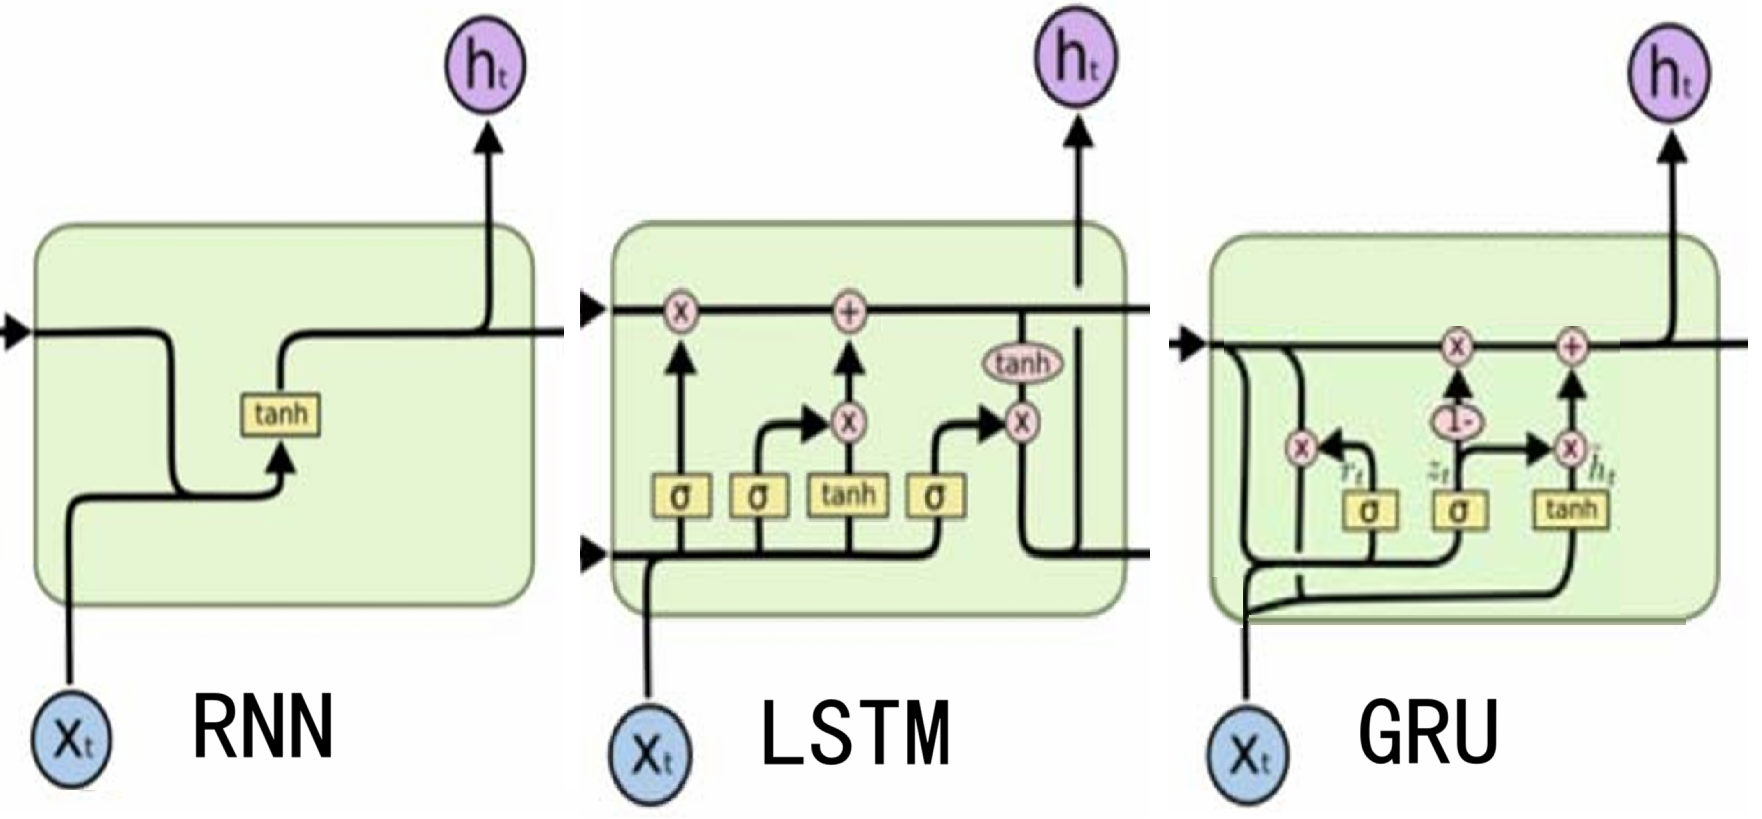
\includegraphics[width=1\linewidth]{image06}
		\label{fig:image06}
	\end{figurehere}
	
	LSTM\textbf{遗忘门}:计算保留比例$f_t=\sigma(\mathbf{W}_f\times[\mathbf{h}_{t-1},\mathbf{x}_t])$
	
	\textbf{输入门}:控制当前候选状态有多少需要往后传递$i_t=\sigma(\mathbf{W}_i\times[\mathbf{h}_{t-1},\mathbf{x}_t])), \tilde{\mathbf{C}}_t = \tanh(\mathbf{W}_C \times [\mathbf{h}_{t-1}, \mathbf{x}_t])$
	
	\textbf{输出门}:控制当前时刻单元状态有多少需要往后输出$o_t = \sigma(\mathbf{W}_o \times [\mathbf{h}_{t-1}, \mathbf{x}_t],~ \mathbf{C}_t = _t \times \mathbf{C}_{t-1} + i_t \times \tilde{\mathbf{C}}_t,~ \mathbf{h}_t = o_t \times \tanh(\mathbf{C}_t)$
	
	GRU\textbf{重置门}:控制前一时刻状态参与候选状态计算的比例$\mathbf{r}_t = \sigma(\mathbf{W}_r \times [\mathbf{h}_{t-1}, \mathbf{x}_t])$替代LSTM中输入门和遗忘门
	
	\textbf{更新门}:控制状态信息的传递比例$\mathbf{z}_t = \sigma(\mathbf{W}_z \times [\mathbf{h}_{t-1}, \mathbf{x}_t])$实现输出门功能
	
	\textbf{候选状态}:$\tilde{\mathbf{h}}_t = \tanh(\mathbf{W} \times [\mathbf{r}_t \times \mathbf{h}_{t-1}, \mathbf{x}_t]),~\mathbf{h}_t = (1 - \mathbf{z}_t) \times \mathbf{h}_{t-1} + \mathbf{z}_t \times \tilde{\mathbf{h}}_t$实现单元状态更新的功能
	
	\subsection*{transformer}
	
	\textbf{注意力}(前馈神经网络):计算效率低
	
	\begin{figurehere}
		\centering
		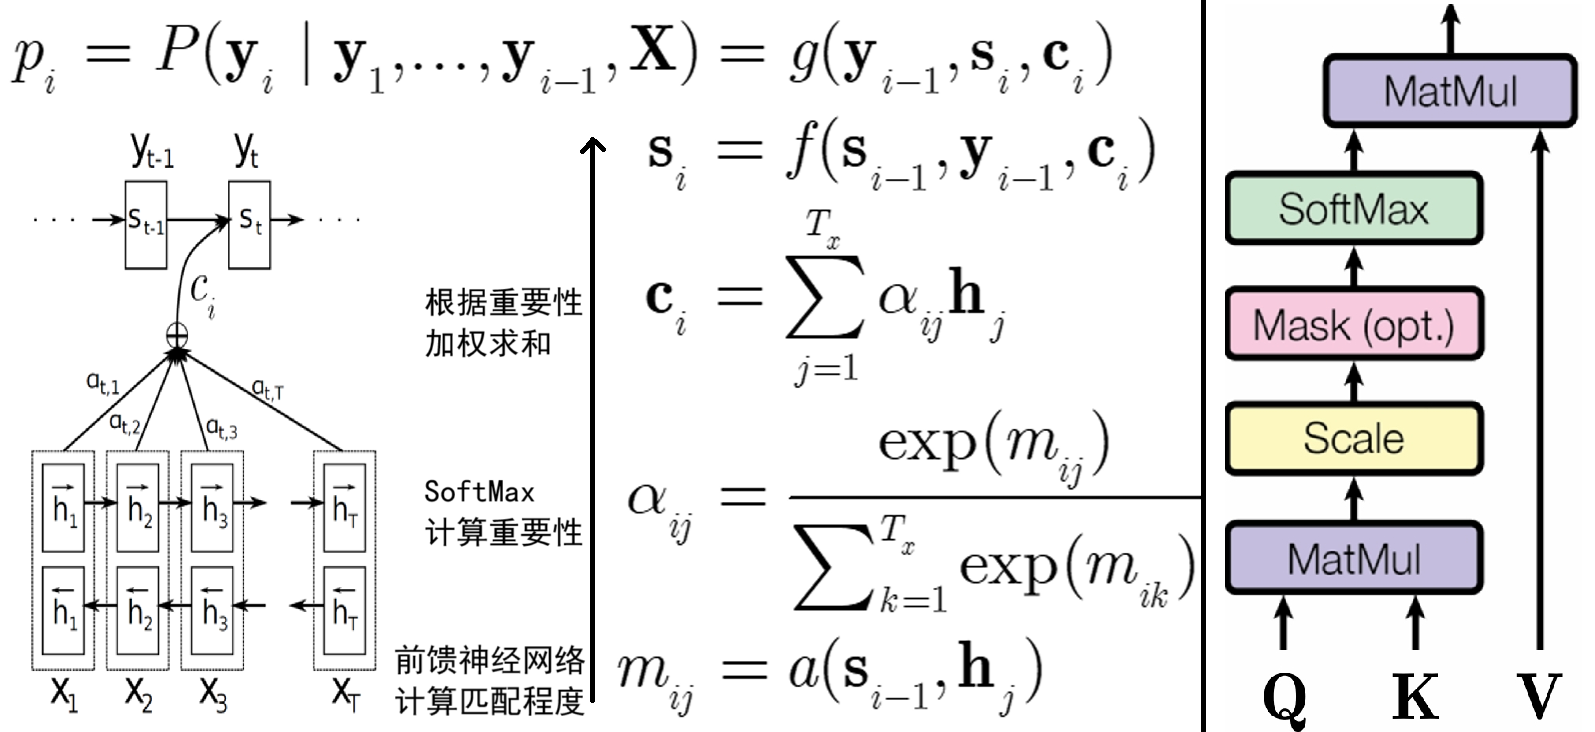
\includegraphics[width=1\linewidth]{image07}
		\label{fig:image07}
	\end{figurehere}
	\textbf{比例点积注意力}:$m_{ij}=a(\mathbf{s}_{i-1},\mathbf{h}_j)$改为$m_{ij}=\mathbf{s}_{i-1}^T\times \mathbf{h}_j$
	
	$\text{Attention}(Q,K,V) = \text{softmax}\left(\frac{QK^T}{\sqrt{d_k}} \right) V \in \mathbb{R}^{m \times d_v}$
	
	$Q \in \mathbb{R}^{m \times d_k},~K \in \mathbb{R}^{n \times d_k},~V \in \mathbb{R}^{n \times d_v}$,复杂度$O(mn)$
	
	\textbf{Softmax置换同变性}:给定置换矩阵 $\mathbf{A} \in \mathbb{R}^{m\times m}$ 和 $\mathbf{B} \in \mathbb{R}^{n\times n}$,任意矩阵 $\mathbf{D} \in \mathbb{R}^{m\times n}$,有$
	\operatorname{softmax}(\mathbf{ADB}) = \mathbf{A} \times \operatorname{softmax}(\mathbf{D}) \times \mathbf{B}$
	
	\textbf{比例点积注意力具有查询置换同变性,键-值对置换不变性}:给定查询矩阵 $\mathbf{Q} \in \mathbb{R}^{m\times d_{k}}$,键矩阵 $\mathbf{K} \in \mathbb{R}^{n\times d_{k}}$,值矩阵 $\mathbf{V} \in \mathbb{R}^{n\times d_{v}}$,置换矩阵 $\mathbf{A} \in \mathbb{R}^{m\times m}$ 和 $\mathbf{B} \in \mathbb{R}^{n\times n}$,有	$	\text{Attention}(\mathbf{AQ}, \mathbf{BK}, \mathbf{BV}) = \mathbf{A} \times \text{Attention}(\mathbf{Q}, \mathbf{K}, \mathbf{V})$
	
	\textbf{掩码注意力}:输入有逻辑顺序时,只能看到之前的输入,不具置换同变性、不变性
	
	\textbf{多头注意力}:将输入$Q,K,V$分别通过$W^{Q},W^{K},W^{V}$投影到不同空间,在每个空间各自计算比例点积注意力;将各个空间的注意力拼接起来,通过矩阵$W^{O}$投影到输出空间
	
	$d_k=d_v=d_model/h=64$,h称为头数
	
	\textbf{自注意力}:$Q,K,V$是同一个矩阵,区别于交叉注意力
	
	\textbf{编码器}:输入嵌入、位置嵌入、多头自注意力(获取输入位置之间的依赖性)、前馈神经网络(捕捉更复杂的特征)、残差网络连接(使用残差学习提升性能)、同隐层标准化(辅助训练)
	
	\textbf{绝对位置编码}:
	
	\begin{figurehere}
		\centering
		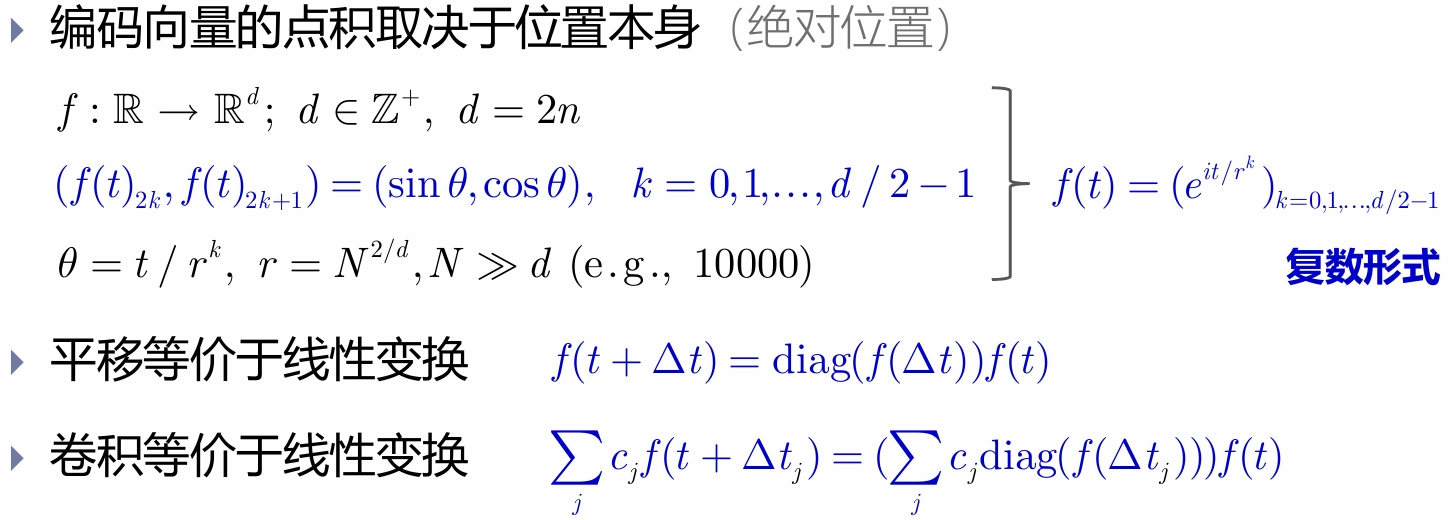
\includegraphics[width=0.7\linewidth]{image08}
		\label{fig:image08}
	\end{figurehere}
	
	\textbf{相对位置编码}:
	
	\begin{figurehere}
		\centering
		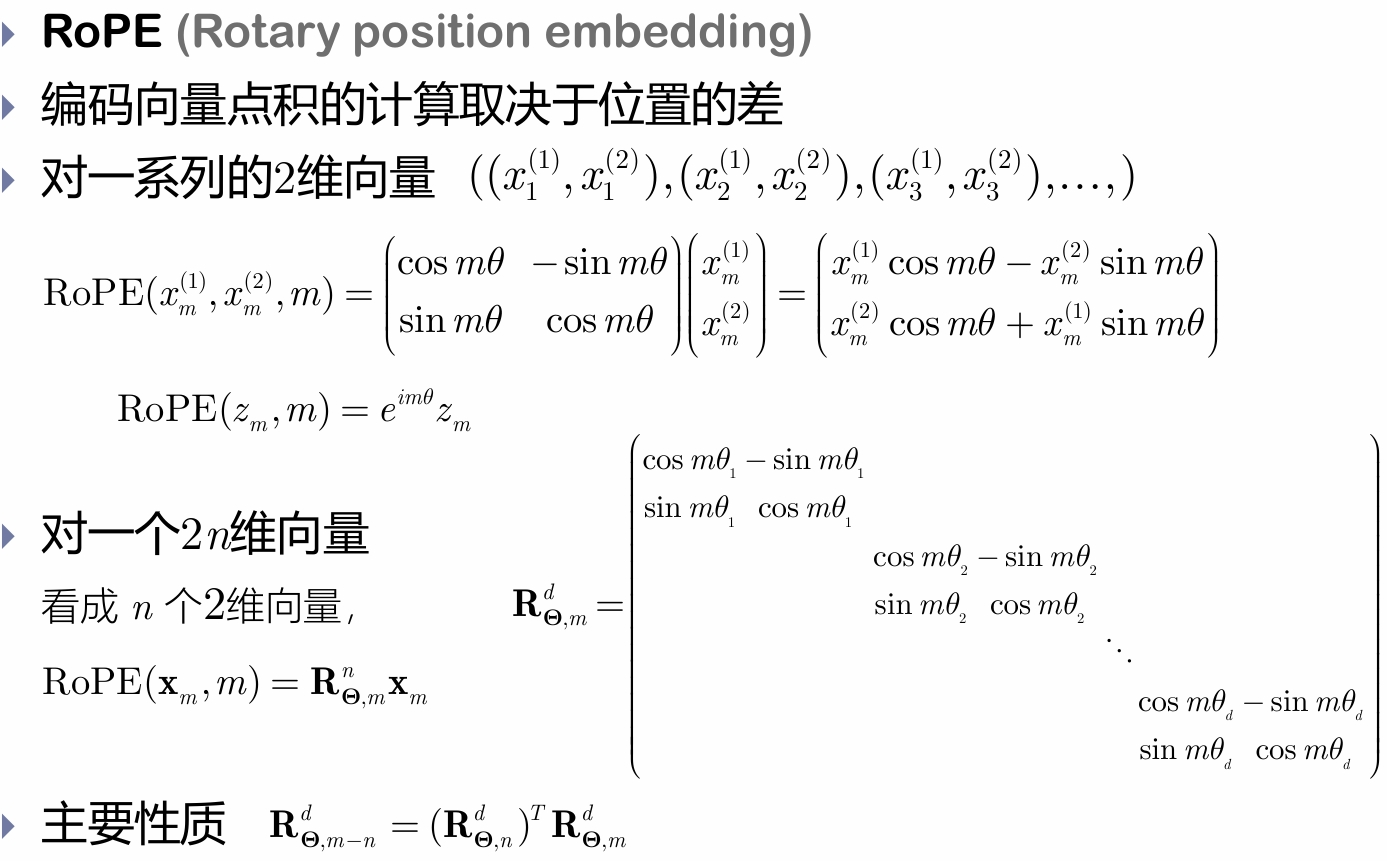
\includegraphics[width=0.7\linewidth]{image09}
		\label{fig:image09}
	\end{figurehere}
	\begin{figurehere}
		\centering
		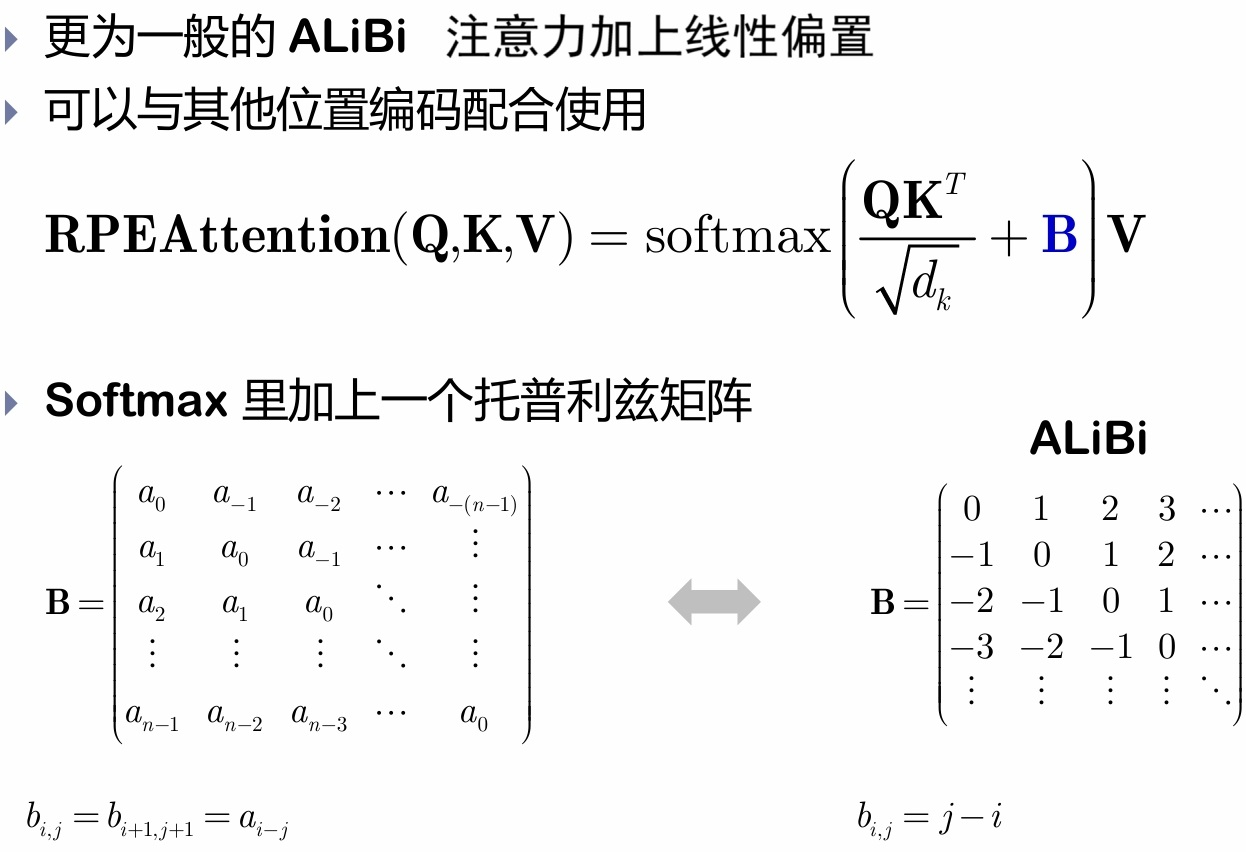
\includegraphics[width=0.7\linewidth]{image10}
		\label{fig:image10}
	\end{figurehere}
	
	
	\textbf{解码器}:掩码自注意力、交叉注意力、概率输出
	
	\section*{四、强化学习}
	
	\subsection*{马尔可夫过程}
	
	\textbf{马尔可夫过程}:二元组$(S,P)$,状态空间$S=\{s_1,...,s_n\}$,状态转移矩阵$P=(p_{ss'})_{n\times n},~p_{ss^{\prime}} = P\left(S_{t+1} = s^{\prime} \mid S_{t} = s\right)$
	
	\textbf{马尔可夫回报过程}:四元组$(S,P,r,\gamma)$
	
	\begin{figurehere}
		\centering
		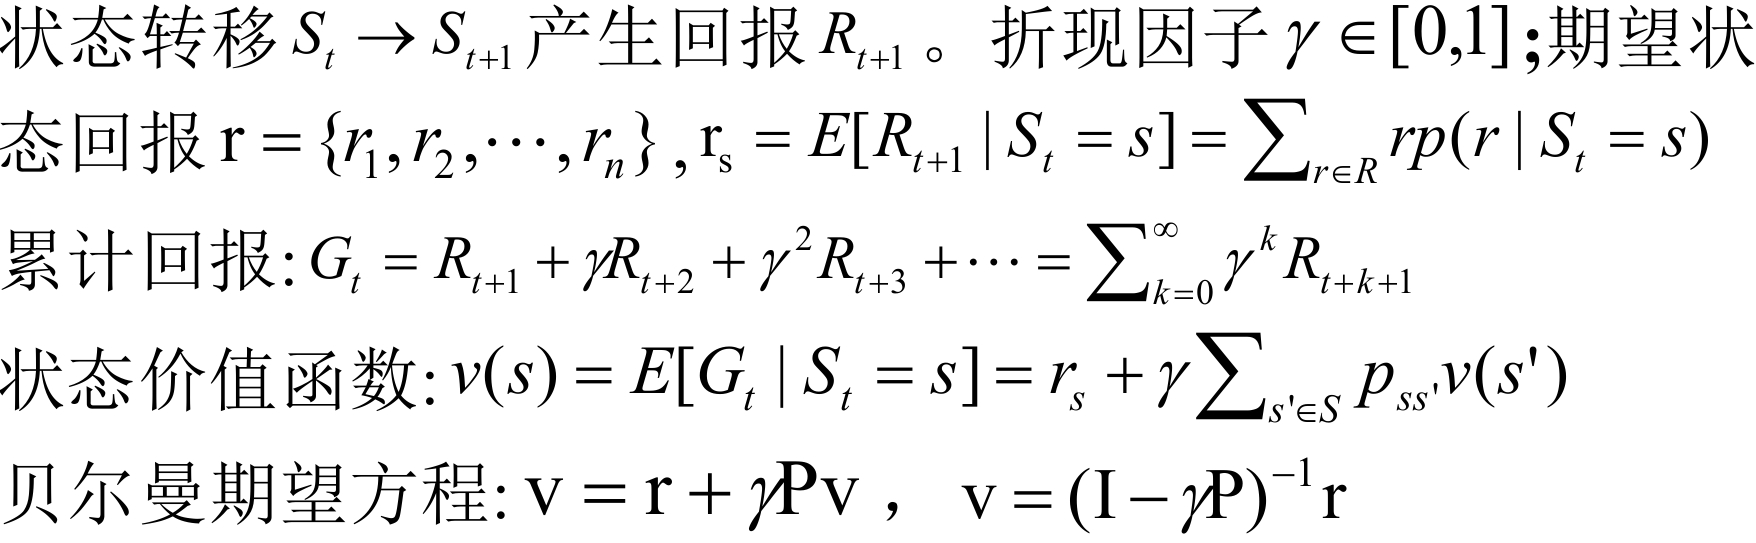
\includegraphics[width=1\linewidth]{image11}
		\label{fig:image11}
	\end{figurehere}
	\textbf{马尔可夫决策过程}:五元组$(S,A,P,R,\gamma)$
	
	行动 $A_{t}$ 导致状态转移 $S_{t}\rightarrow S_{t+1}$ 产生回报 $R_{t+1}$。
	
	行动空间:$A=\{a_{1},a_{2},\cdots,a_{m}\}$;状态转移:$P=(p_{ss^{\prime}}^{a})_{n\times n\times m}$ 其中 $p_{ss^{\prime}}^{a}=P(S_{t+1}=s^{\prime}|S_{t}=s,A_{t}=a)=\sum_{r\in R}p(s^{\prime},r|s,a)$
	
	行动期望回报 $R=(r_{s}^{a})_{n\times m}$, $r_{s}^{a}=E[R_{t+1}|S_{t}=s,A_{t}=a]=\sum_{r\in R}r\sum_{s^{\prime}\in S}p(s^{\prime},r|s,a)$。
	
	策略:$\pi(a|s)=P(A_{t}=a|S_{t}=s)$(s下选a的概率),$p^{\pi}(S_{t+1}=s^{\prime}|S_{t}=s)=\sum_{a\in A}\pi(a|s)p_{ss^{\prime}}^{a}$,$r_{s}^{\pi}=\sum_{a\in A}\pi(a|s)r_{s}^{a}$。
	
	状态价值:$v_{\pi}(s)=E[G_{t}|S_{t}=s]=\sum_{a\in A}\pi(a|s)q_{\pi}(s,a)$
	
	行动价值(后续状态加权和):$q_{\pi}(s,a)=E[G_{t}|S_{t}=s,A_{t}=a]=r_{s}^{a}+\gamma\sum_{s^{\prime}\in S}p_{ss^{\prime}}^{a}v_{\pi}(s^{\prime})$
	
	*状态价值是行动价值的期望;行动价值是行动即时回报与后续状态价值折扣之和的期望
	
	*量化评价一个策略—预测问题;寻找最优策略—控制问题
	
	\textbf{贝尔曼期望方程}:
	
	状态方程$v_{\pi}(s)=\sum_{a\in A}\pi(a|s)\left(r_{s}^{a}+\gamma\sum_{s^{\prime}\in S}p_{ss^{\prime}}^{a}v_{\pi}(s^{\prime})\right)$
	
	行动方程$q_{\pi}(s, a)=r_{s}^{a}+\gamma\sum_{s^{\prime}\in S}p_{ss^{\prime}}^{a}\sum_{a^{\prime}\in A}\pi(a^{\prime}|s^{\prime})q_{\pi}(s^{\prime},a^{\prime})$
	
	最优状态价值: $v_{*}(s)=\max_{\pi} v_{\pi}(s)=v_{\pi_{*}}(s)$
	
	最优行动价值: $q_{*}(s,a)=\max_{\pi} q_{\pi}(s,a)=q_{\pi_{*}}(s,a)$
	
	关系式: $v_{*}(s)=\max_{a\in A}q_{*}(s,a)$
	
	最优策略(贪心): $\pi_{*}(a|s)=\mathbb{1}_{a=\arg\max q_{*}(s,a)}$
	
	状...最优方程:$v_*(s)=\max_{a\in\mathbf{A}}\left(r_s^a+\gamma\sum_{s'\in\mathbf{S}}p_{ss'}^av_*(s')\right)$
	
	期望形式:$v_*(s)=\max_{a\in\mathbf{A}}\mathrm{E}[R_{t + 1}+\gamma v_*(S_{t + 1})|S_t = s,A_t = a]$
	
	行...最优方程:$q_*(s,a)=r_s^a+\gamma\sum_{s'\in\mathbf{S}}p_{ss'}^a\max_{a\in\mathbf{A}}q_*(s',a)$
	
	$q_*(s,a)=\mathrm{E}[R_{t + 1}+\gamma\max_{a_{t + 1}\in\mathbf{A}}q_*(S_{t + 1},a_{t + 1})|S_t = s,A_t = a]$
	
	\textbf{策略评价}:计算价值函数的值(法1解方程组见上,法2迭代求解$v^{(k+1)}=r^{\pi}+\gamma P^{\pi} v^{(k)}$即$v_{k+1}(s)=r_{s}^{\pi}+\gamma\sum_{s^{\prime}\in S}p_{ss^{\prime}}^{\pi} v_{k}(s^{\prime})$
	
	*求得状态价值后,直接计算行动价值
	
	\textbf{策略改进}:$\pi_{k+1}(s)=\arg\max_{\pi(s)}\left(r_{s}^{\pi(s)}+\gamma\sum_{s^{\prime}\in\mathbf{S}}p_{ss^{\prime}}^{\pi(s)}v_{\pi_{k}}\left(s^{\prime}\right)\right)$即$\pi_{k+1}=\arg\max_{\pi}\left(\mathbf{r}_{\pi}+\gamma\mathbf{P}_{\pi}\mathbf{v}_{\pi_{k}}\right)$直至收敛
	
	\textbf{策略迭代}:交替进行\textbf{策略评价}与\textbf{策略改进},求解最优策略
	
	\textbf{价值迭代}:计算价值函数的\textbf{最大值}
	
	$v_{k+1}(s)=\max_{a\in A}\left(r_{s}^{\pi}+\gamma\sum_{s^{\prime}\in S}p_{ss^{\prime}}^{\pi}v_{k}(s^{\prime})\right)$即$\mathbf{v}_{k+1}=\max_{a \in \mathbf{A}}\left(\mathbf{r}^a+\gamma\mathbf{P}^a\mathbf{v}^{(k)}\right)$直至收敛
	
	*求解后可进一步确定最优策略$\pi_{*}(s)=\arg\max_{a\in\mathbf{A}} q_{*}(s,a)=\arg\max_{a\in\mathbf{A}}\left(r_{s}^{a}+\gamma\sum_{s^{\prime}\in\mathbf{S}} p_{ss^{\prime}}^{a} v_{*}\left(s^{\prime}\right)\right)$
	
	\textbf{同步迭代}:算完所有s更新一次策略,留两份价值,计算量大收敛慢
	
	\textbf{异步迭代}:算完一个s就更新一次策略,计算量小收敛快
	
	\subsection*{蒙特卡洛}
	P矩阵未知时状态价值预测、策略改进——均值近似数学期望
	
	\textbf{蒙特卡洛积分}:$\mathrm{E}_{p(x)}[f(X)]=\int_{-\infty}^{\infty} f(x)p(x)dx\approx\frac{1}{n}\sum_{i=1}^{n} f\left(x_{i}\right)$
	
	\textbf{蒙特卡洛预测}
	
	\textbf{首次访问蒙特卡洛}:根据待评价策略产生观测片段$s_{1},a_{1},r_{2},\ldots,s_{t},a_{t},r_{t+1},\ldots,s_{T},a_{T},r_{T+1}$,当$s_{t}=s$时,检查之前是否出现过,计算$g_{i}=r_{t+1}+\gamma r_{t+2}+\cdots+\gamma^{T-t}r_{T+1}$,重复$n$次得到$g_{1},g_{2},\ldots,g_{n}$,最终状态价值估计为$v(s_{t})=\frac{1}{n}\sum_{i=1}^{n}g_{i}$。
	
	\textbf{每次访问蒙特卡洛}:只要观测片段出现目标状态,都用来计算平均值
	
	*均需仿真到终止状态,仅适用于分幕式\textbf{马尔可夫决策过程}
	
	增量式蒙特卡洛:$V(S_{t})\leftarrow V(S_{t})+\frac{1}{k}(G_{t}-V(S_{t}))$,$k\leftarrow k+1$
	
	定步长蒙特卡洛:$V(S_{t})\leftarrow V(S_{t})+\alpha(G_{t}-V(S_{t}))$
	
	无模型行动价值预测:$q_{\pi}(s,a)\approx \frac{1}{n}\sum G_{i}$
	
	增量式Q学习:$Q(S_{t},A_{t})\leftarrow Q(S_{t},A_{t})+\frac{1}{k}(G_{t}-Q(S_{t},A_{t}))$,$k\leftarrow k+1$
	
	定步长Q学习:$Q(S_{t},A_{t})\leftarrow Q(S_{t},A_{t})+\alpha(G_{t}-Q(S_{t},A_{t}))$
	
	\textbf{蒙特卡洛控制}:策略评价和策略改进交替进行
	
	策略改进:$\pi^{\prime}(S_{t})=\arg\max_{a\in A}Q(S_{t},a)$
	
	$\varepsilon-$贪心策略:$\pi_{*}(a\mid s)=\begin{cases}1-\varepsilon+\varepsilon/m, & a=\arg\max q_{*}(s,a)\\ \varepsilon/m, & \text{其他情况}\end{cases}$
	
	对比:\textbf{动态规划}有模型不采样不需要有终止状态计算量与状态数量相关像宽搜;\textbf{蒙特卡洛}无模型要采样需要有终止状态计算量与状态数量无关像深搜
	
	\subsection*{时序差分}
	P矩阵未知时,从部分序列学习
	
	\textbf{时序差分预测}:$G_{t+1}$用$\gamma v_t(s_{t+1})$估计
	
	\textbf{状态价值迭代}$v_{t+1}(s_{t})=v_{t}(S_{t})+\alpha_{t}(r_{t+1}+\gamma v_{t}(s_{t+1})-v_{t}(s_{t}))$
	
	\textbf{行动价值迭代}$q_{t+1}(s_t, a_t) = q_t(s_t, a_t) + \alpha_t(r_{t+1} + \gamma q_t(s_{t+1}, a_{t+1}) - q_t(s_t, a_t))$
	
	对比:\textbf{蒙特卡洛}完整序列终止分幕非马;\textbf{时序差分}不完整序列持续连续马尔可夫场景
	
	\textbf{行为策略}:产生经验轨迹;\textbf{目标策略}:算法试图优化
	
	\textbf{时序差分控制}:同轨On policy两者同(SARSA蒙特卡洛);离轨Off policy两者分离(ESARSA和Q学习)
	
	\begin{figurehere}
		\centering
		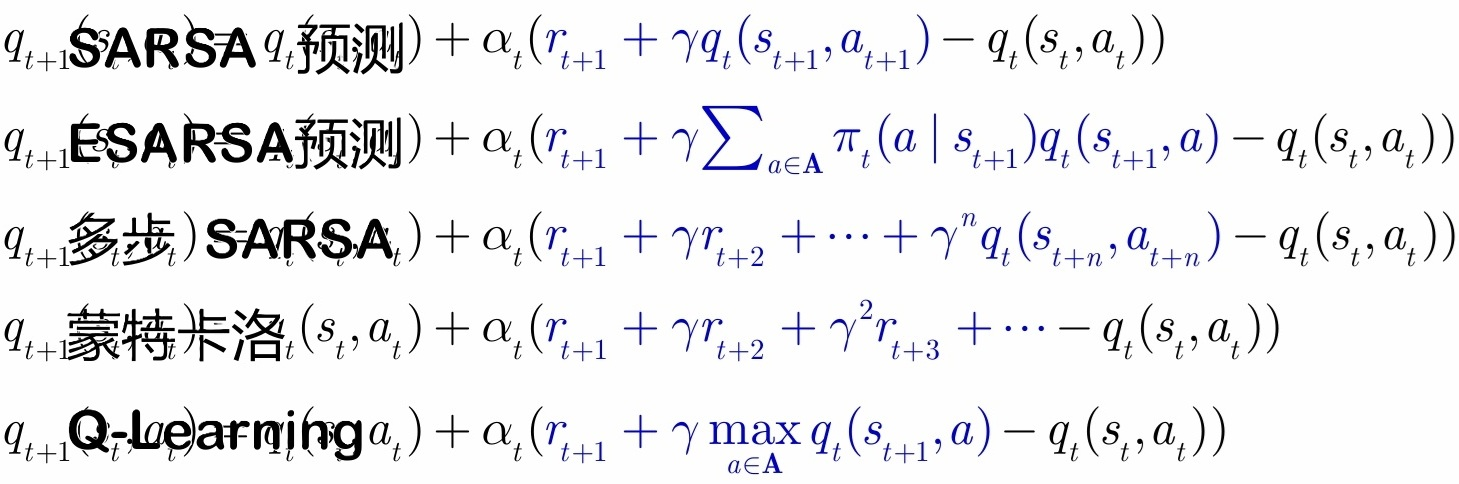
\includegraphics[width=1\linewidth]{image12}
		\label{fig:image12}
	\end{figurehere}
	\textbf{解释}:SARSA:行为策略和目标策略都是greedy-$\varepsilon$
	
	Q-learning:行为策略greedy-$\varepsilon$目标策略greedy
	
	E-SARSA:行为策略greedy-$\varepsilon$目标策略行动期望
	
	\begin{figurehere}
		\centering
		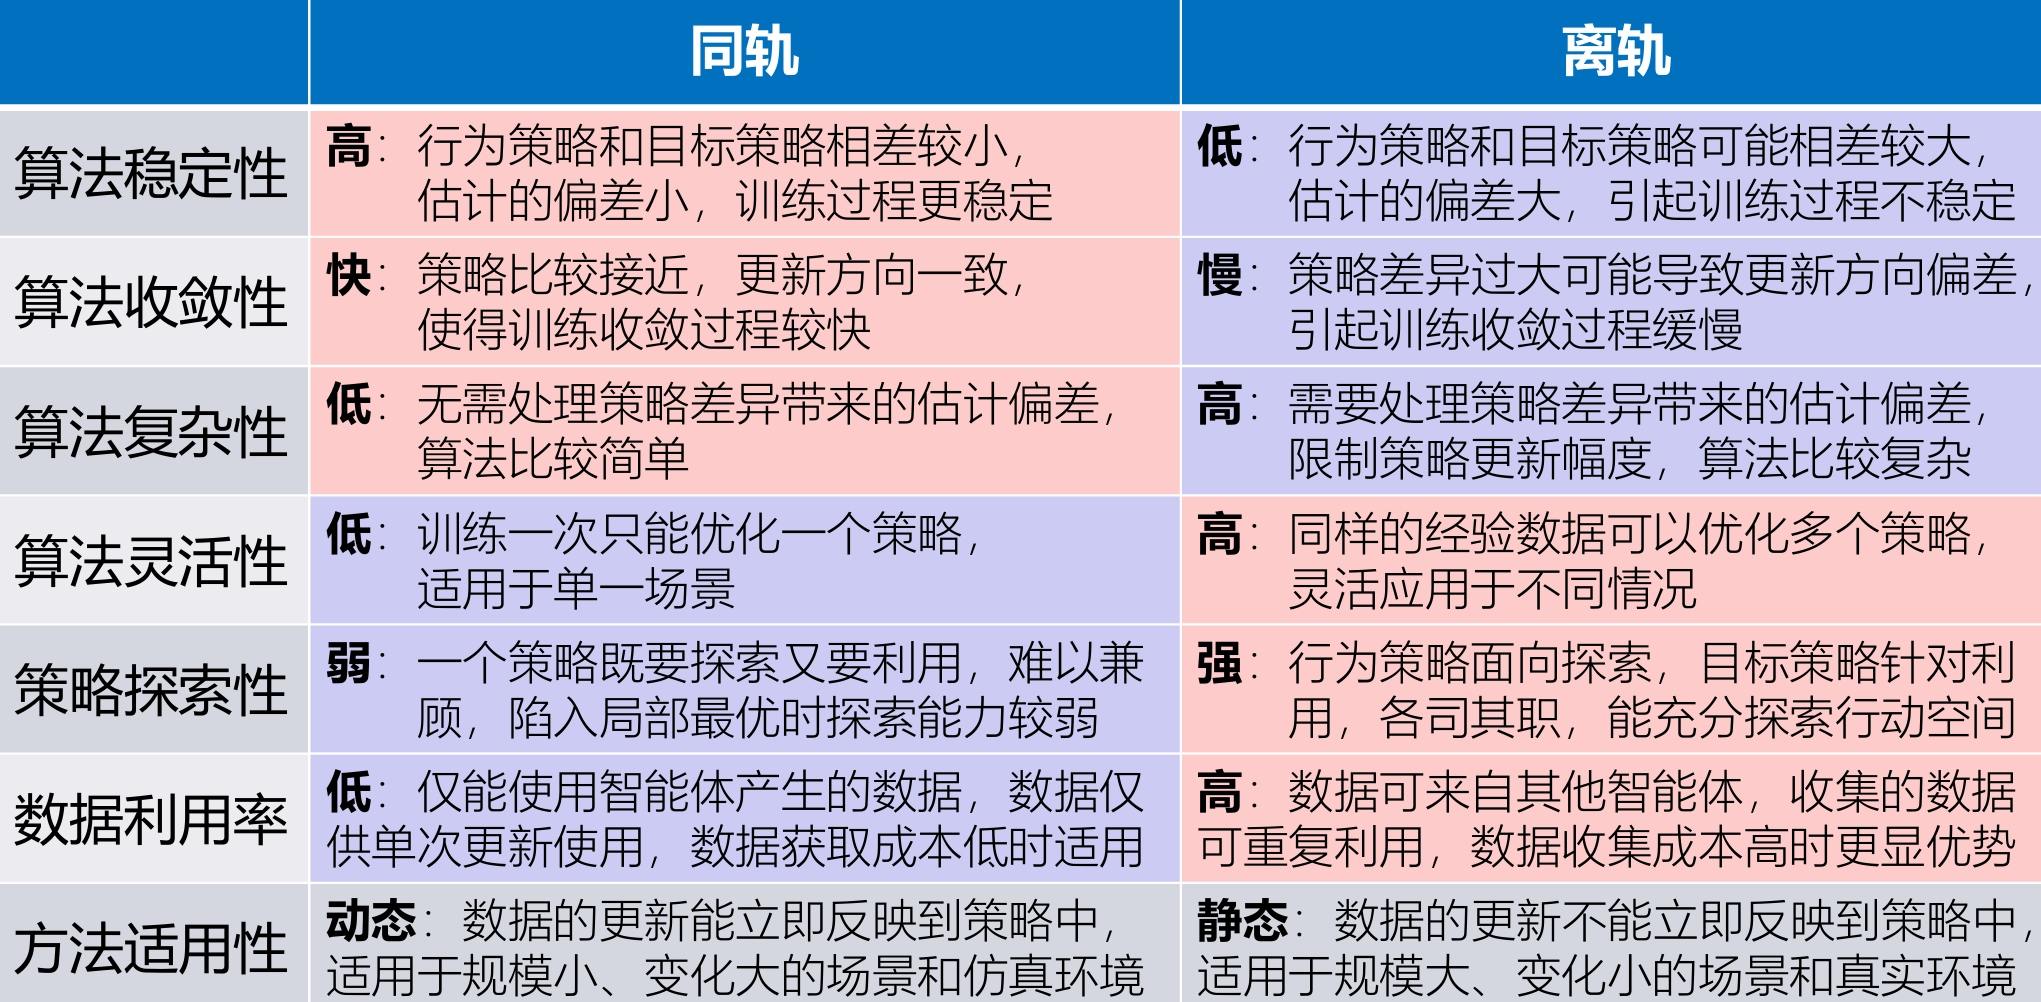
\includegraphics[width=1\linewidth]{image13}
		\label{fig:image13}
	\end{figurehere}
	\begin{figurehere}
		\centering
		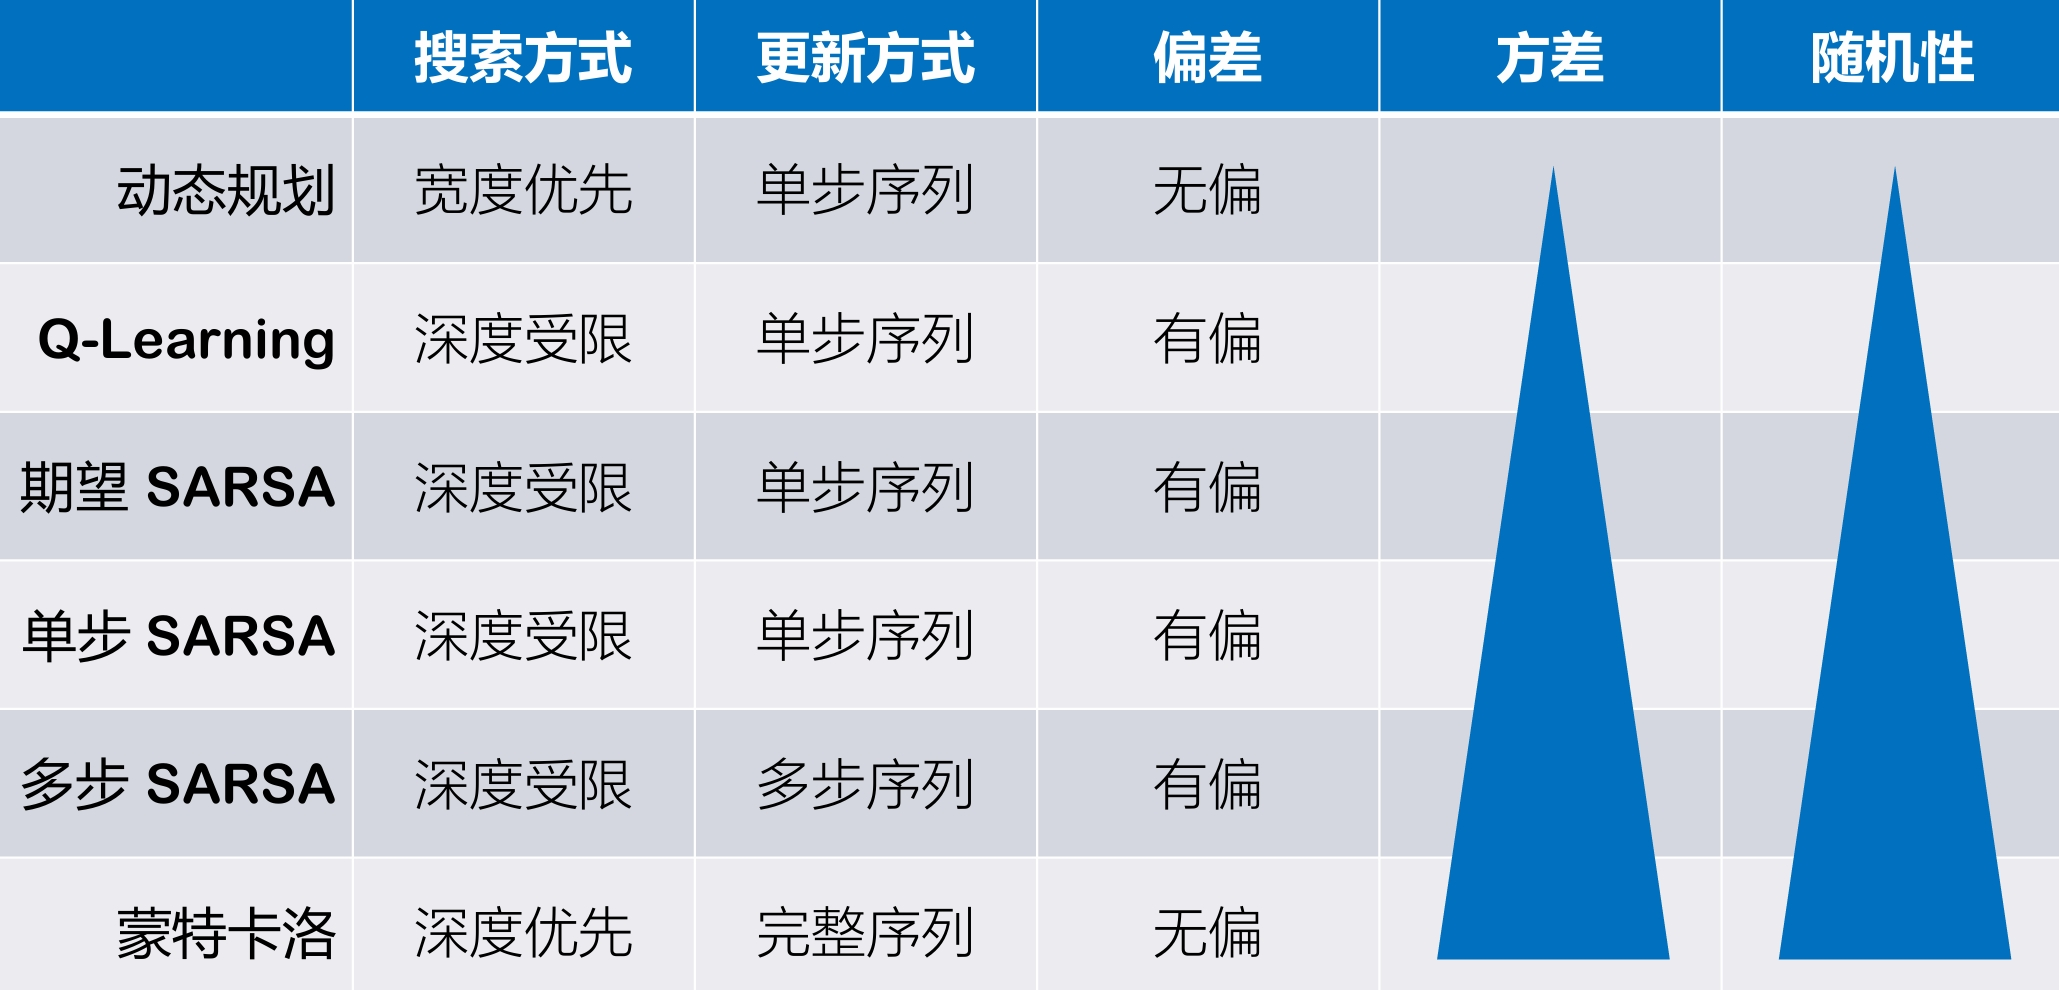
\includegraphics[width=1\linewidth]{image14}
		\label{fig:image14}
	\end{figurehere}
	
	\subsection*{价值近似}
	以上统称表格法:当状态/行动数量过多时,算不动且泛化性差$\rightarrow$用参数化模型近似价值函数(监督学习)
	
	\textbf{状态价值近似}:
	
	\textbf{1.价值模型}:线性$v_\pi(s)\approx\hat{v}(s, w)=w^T\phi(s)$,这里$w^T$为参数向量,$\phi(s)$为特征向量(特征提取用傅里叶基函数等方法);NN$v_\pi(s)\approx\hat{v}(s, w)=\text{Value Network}$非线性建模,模型容量大,因此可以逼近非常复杂的价值函数
	
	\textbf{2.优化目标}:$J(w)=E\left[\left(v_{\pi}(S)-\hat{v}(S, w)\right)^2\right]=\sum_{s\in S} d(s)\left(v_{\pi}(s)-\hat{v}(s, w)\right)^2$,其中$d(s)$是状态服从的分布(均匀$d_0(s)=\frac{1}{|S|}$;马尔可夫稳态$d^T=d^T P$更合理)
	
	\textbf{3.优化方法}:
	
	SGD方法$w_{t+1}=w_t+\alpha_t\left(v_{\pi}\left(s_t\right)-\hat{v}\left(s_t, w_t\right)\right)\nabla_{w} \hat{v}\left(s_t, w_t\right)$
	
	蒙特卡洛$w_{t+1}=w_t+\alpha_t\left(g_t-\hat{v}\left(s_t, w_t\right)\right)\nabla_{w} \hat{v}\left(s_t, w_t\right)$
	
	时分$w_{t+1}=w_t+\alpha_t\left(r_{t+1}+\gamma\hat{v}\left(s_{t+1}, w_t\right)-\hat{v}\left(s_t, w_t\right)\right)\nabla_{w} \hat{v}\left(s_t, w_t\right)$
	
	\textbf{行动价值近似}:
	
	\textbf{1.价值模型}:$q_\pi(s, a)\approx\hat{q}(s, a, w)$
	
	\textbf{2.优化目标}:$J(w)=E\left[\left(q_\pi(S, A)-\hat{q}(S, A, w)\right)^2\right]$
	
	\textbf{3.优化方法}:
	
	蒙特卡洛$\mathbf{w}_{t+1} = \mathbf{w}_t + \alpha_t(g_t - \hat{q}(s_t,a_t,\mathbf{w}_t))\nabla_{\mathbf{w}}\hat{q}(s_t,a_t,\mathbf{w}_t)$
	
	SARSA$~\mathbf{w}_{t+1} = \mathbf{w}_t + \alpha_t(r_{t+1} + \hat{q}(s_{t+1},a_{t+1},\mathbf{w}_t) - \hat{q}(s_t,a_t,\mathbf{w}_t))\nabla_{\mathbf{w}}\hat{q}(s_t,a_t,\mathbf{w}_t)$
	
	Q-Learning$~\mathbf{w}_{t+1} = \mathbf{w}_t + \alpha_t(r_{t+1} + \max_{a\in\mathbf{A}}\hat{q}(s_{t+1},a,\mathbf{w}_t) - \hat{q}(s_t,a_t,\mathbf{w}_t))\nabla_{\mathbf{w}}\hat{q}(s_t,a_t,\mathbf{w}_t)$
	
	\subsection*{策略梯度}
	对策略建立参数化模型(给出随机策略,实现柔性控制;灵活性收敛性更好)
	
	\textbf{1.策略模型}:线性+Softmax$\pi(a\mid s)\approx\pi(a\mid s,\theta)=\frac{\exp(h(s, a,\theta))}{\sum_{s, a}\exp(h(s, a,\theta))}$,其中$h(s, a,\theta)=\theta^T\phi(s, a)$($\theta^T$为参数向量,$\phi(s)$为特征向量);NN:$\pi(a\mid s)\approx\pi(a\mid s,\theta)=\text{Policy Network}$模型容量大
	
	\textbf{2.优化目标}:MAX平均状态价值$J(\theta)=\bar{v}_{\pi}=E_{s\sim d}\left[v_{\pi}(S)\right]=\sum_{s\in S} d(s) v_{\pi}(s)=d^T v_{\pi}$【$d(s)$与策略无关时选均匀分布$d_0(s)=\frac{1}{|S|}$;其次是仅考虑某一个特殊状态(例如初始状态)的价值,即$\bar{v}_\pi=v_\pi\left(s_0\right)$;与策略相关时常选稳态分布满足$\mathbf{d}_\pi^T=\mathbf{d}_\pi^T \mathbf{P}_\pi$】;MAX平均即时回报$J(\theta)=\bar{r}_\pi=E\left[r_\pi(S)\right]=\sum_{s\in S} d(s) r_\pi(s)=d^T r_\pi$。这里,状态的即时回报以向量表示$r_\pi=\left(\ldots, r_\pi(s),\ldots\right)^T$,由贝尔曼期望方程$v_{\pi}=r_{\pi}+\gamma P_{\pi} v_{\pi}$,两个目标等价
	
	\textbf{3.最优策略}:策略梯度定理$\nabla_{\theta} J(\theta)=\sum_{s\in S}\eta(s)\sum_{a\in A}\nabla_{\theta}\pi(a\mid s,\theta) q_{\pi}(s, a)=E_{S\sim\eta}\left[\sum_{a\in A}\nabla_{\theta}\pi(a\mid S,\theta) q_{\pi}(S, a)\right]=E_{S\sim\eta, A\sim\pi}\left[\nabla_{\theta}\ln\pi(A\mid S,\theta) q_{\pi}(S, A)\right]$
	
	\textbf{全部行动算法}:随机梯度上升,期望用采样代替,只对状态采样$\nabla_{\theta} J(\theta)\approx E_{A\sim\pi}\left[\nabla_{\theta}\ln\pi\left(A\mid s_t,\theta\right) q_{\pi}\left(s_t, A\right)\right]=\sum_{a\in A}\nabla_{\theta}\pi\left(a\mid s_t,\theta_t\right) q_t\left(s_t, a\right)$
	
	\textbf{REINFORCE算法}:蒙特卡洛对状态和行动都采样,基于当前策略$\pi\left(a\mid s,\theta_t\right)$与环境交互,采样产生序列$s_1, a_1, r_2,\ldots, s_t, a_t, r_{t+1},\ldots, s_T, a_T, r_{T+1}$,利用该序列估计行动价值$g_i=r_{t+1}+\gamma r_{t+2}+\cdots+\gamma^{T-t} r_{T+1}$,然后更新策略$\theta_{t+1}=\theta_{t}+\alpha_{t}\nabla_{\theta}\ln\pi\left(a_{t}\mid s_{t},\theta_{t}\right) q_{t}\left(s_{t}, a_{t}\right)$
	
	等价形式:$\pi(a_t\mid s_t,\theta_{t+1})\approx\pi(a_t\mid s_t,\theta_t)+\alpha_t\beta_t\left\|\nabla_{\theta}\pi(a_t\mid s_t,\theta_t)\right\|^2$,其中$\beta_t=\frac{q_t\left(s_t, a_t\right)}{\pi\left(a_t\mid s_t,\theta_t\right)}$——鼓励利用:策略改进的方向/幅度取决于$q_t\left(s_t, a_t\right)$符号/绝对值;鼓励探索:$\beta_t$与行动概率$\pi\left(a_t\mid s_t,\theta\right)$成反比
	
	\subsection*{行动器-评判器}
	用时序差分计算价值的策略梯度法,效果最好最常使用
	
	\textbf{QAC}:SARSA中$\varepsilon$-贪心变为策略梯度
	
	\textbf{改进1利用策略梯度的基线不变性引入优势函数,降低估计量的方差}:
	
	$\nabla_{\theta} J(\theta)=E_{S\sim\eta, A\sim\pi}\left[\nabla_{\theta}\ln\pi(A\mid S,\theta) q_{\pi}(S, A)\right]=E_{S\sim\eta, A\sim\pi}\left[\nabla_{\theta}\ln\pi(A\mid S,\theta)\left(q_{\pi}(S, A)-b(S)\right)\right]$
	
	行动价值减基线值,策略梯度不变,方差减小;常用$b(S)=v_{\pi}(S)$
	
	\textbf{优势函数}:行动价值减去基线,如$\delta_t\left(s_t, a_t\right)=q_t\left(s_t, a_t\right)-v_t\left(s_t\right)$
	
	\textbf{解释}:优势函数是采样的行动价值与它的均值做比较,比与0比较合理
	
	\textbf{改进2利用时序差分降低模型的复杂度}:$\delta_t\left(s_t\right)=q_t\left(s_t, a_t\right)-v_t\left(s_t\right)=r_{t+1}+\gamma v_t\left(s_{t+1}\right)-v_t\left(s_t\right)$,不需要算行动价值了
	
	\textbf{经典算法A2C}:
	
	\begin{figurehere}
		\centering
		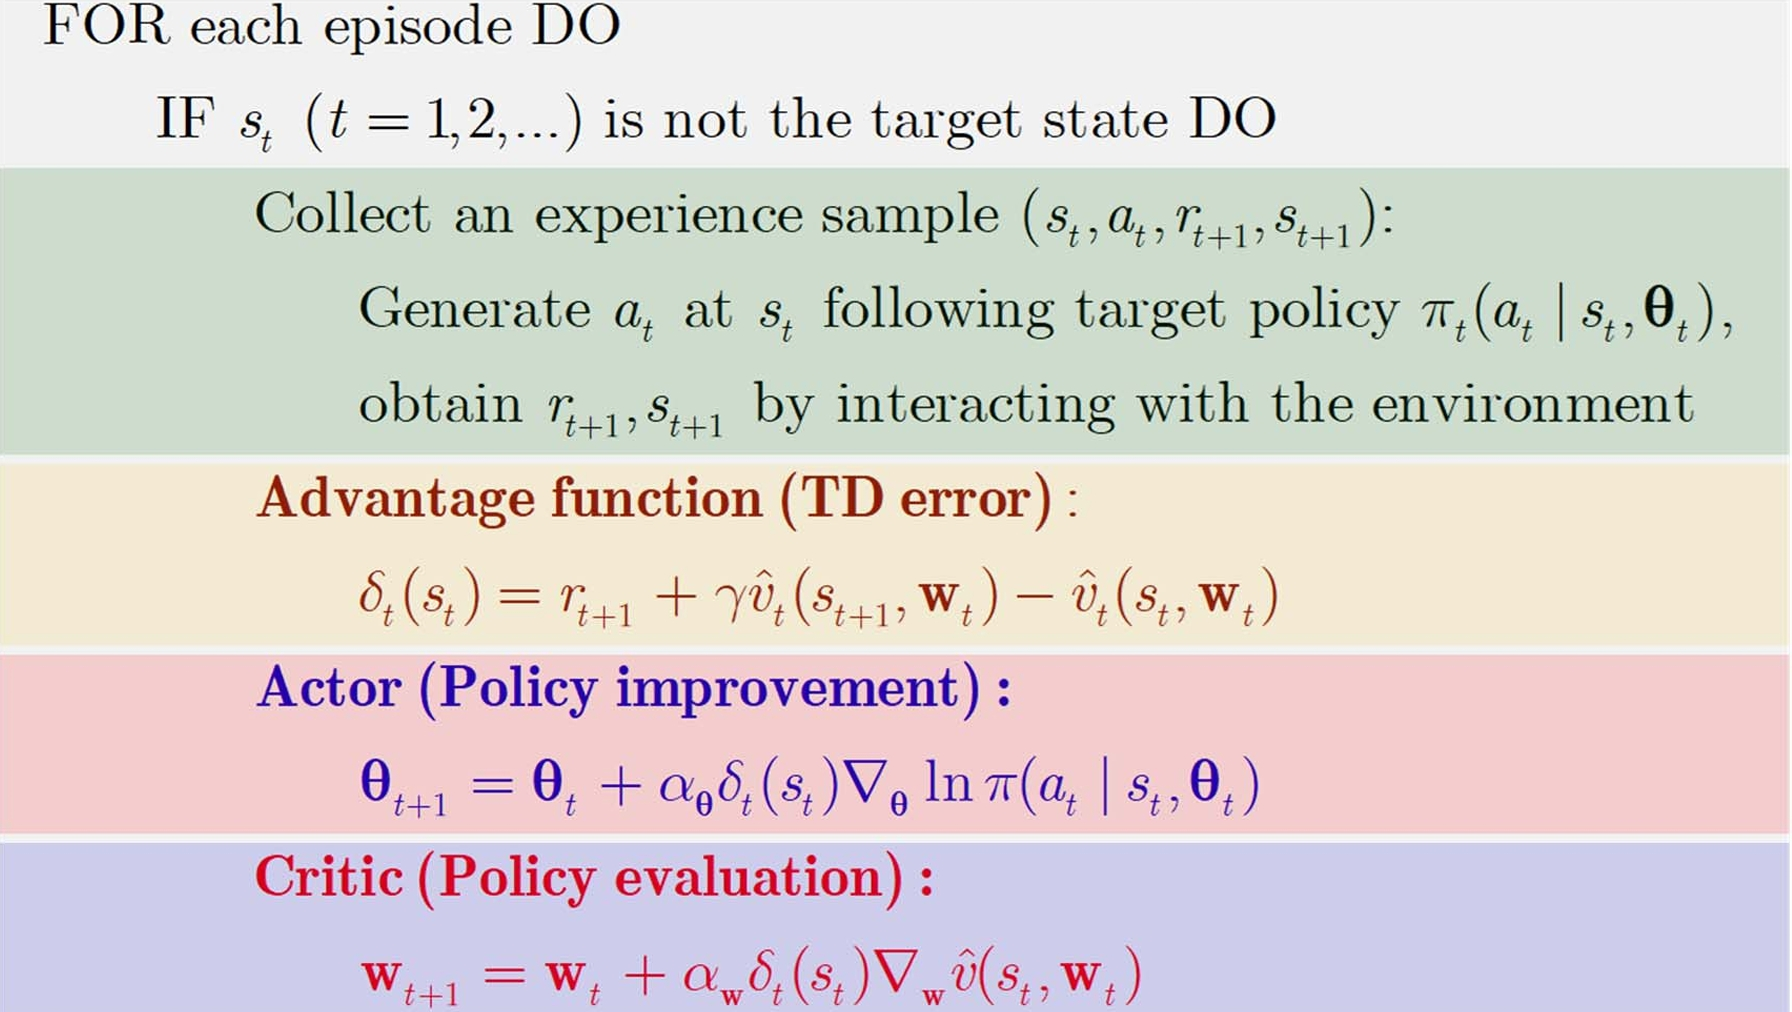
\includegraphics[width=1\linewidth]{image15}
		\label{fig:image15}
	\end{figurehere}
	\textbf{改进3:通过重要性采样转换为离轨学习}:
	
	\textbf{重要性采样}:$E_{X\sim T}[X]=E_{X\sim B}\left[\frac{p_T(x)}{p_B(x)} X\right]$
	
	\begin{figurehere}
		\centering
		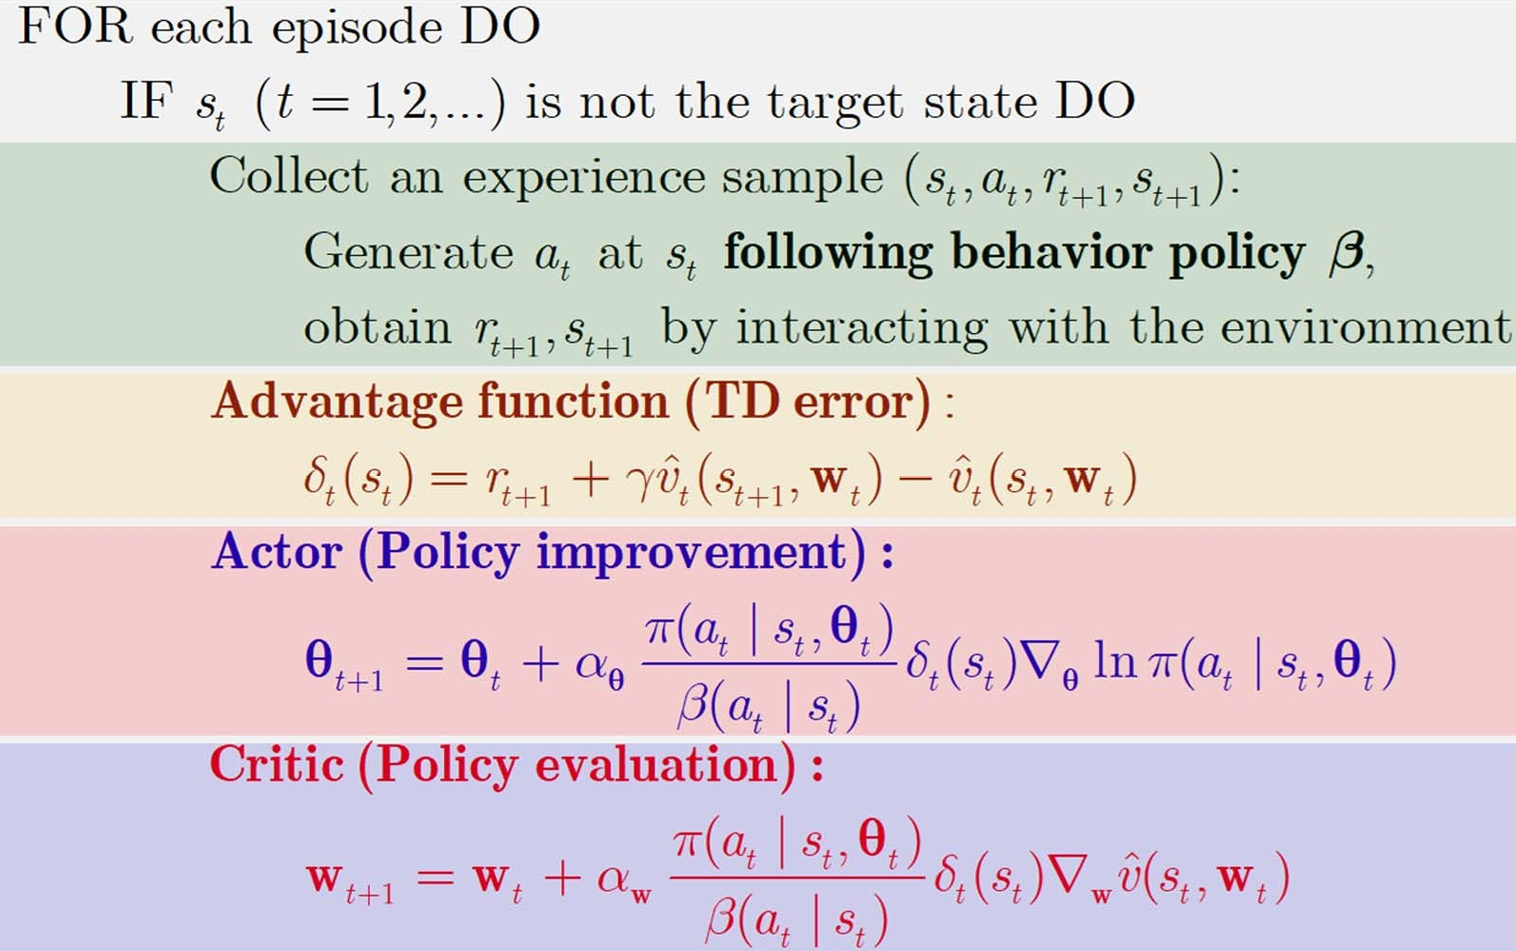
\includegraphics[width=1\linewidth]{image16}
		\label{fig:image16}
	\end{figurehere}
	
	